\documentclass{article}
\usepackage{graphicx} % Required for inserting images
\graphicspath{ {./images/} }
\usepackage[square,numbers]{natbib}
\usepackage[letterpaper,top=2cm,bottom=2cm,left=3cm,right=3cm,marginparwidth=1.75cm]{geometry}
\usepackage{hyperref}
\usepackage{placeins}

\bibliographystyle{dinat}


\begin{document}


\title{Unit 13}
\author{Chris Hadden}
\date{}
\maketitle

\section{P6 Target Audience for the Pampered Pets Campaign}
Pampered Pets have identified what channels would give them the most impact, and what channels customers also want to use to reach out to brands. From this we now want to focus in on the target audience Pampered Pets should be looking at.

\section{Market Segmentation Analysis}
There are a number of ways of splitting up your target audience and researching what how sections respond to your market area. We will work through this.

\subsection{Age}
It is always worth seeing how your target market may break down by age. 

Looking at SproutSocial's breakdown of social media user age range \cite{sproutage}
\begin{center}
    \begin{tabular}{||c c c c||} 
     \hline
     Age & Top & Middle & Bottom \\ [0.5ex] 
     \hline\hline
     18-29 & Snapchat (41\%) & TikTok (35\%) & Instagram (32\%) \\ 
     \hline
     30-39 & LinkedIn (34\%), & X/Twitter (34\%) & Snapchat (33\%) \\
     \hline
     40-49 & LinkedIn (25\%) & Facebook (22\%) & X/Twitter (21\%) \\
     \hline
     50-59 & Facebook (29\%) & LinkedIn (24\%) & Pinterest (24\%) \\
     \hline
    \end{tabular}
    \label {Age ranges of social media}
    \end{center}

We can see that Facebook covers the majority of people in the age range 40 to 59 and Snapchat covers most people in the age range 18-39. This gives us quite a good place to start.

Another way of looking at age is to see what pets each age range owns. As we can see from figure \ref{fig:pets} from Forbes \cite{ownersage} there isn't a lot in the age differences, which is reassuring in a way, at least there's no specific age range to target and from what we have seen from the social media platforms it seems like there a few that cover most age ranges.

\FloatBarrier
\begin{figure}[ht]
    \caption{Pet Ownership by Pet}
    \centering
    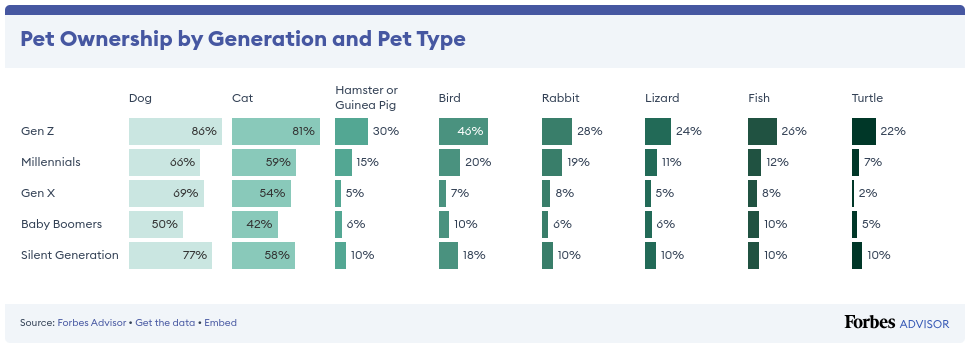
\includegraphics[width=0.8\textwidth]{OwnersByAge}
    \label{fig:pets}
    \end{figure}
    \FloatBarrier

\subsection{Other factors}
A study by Inforgroup in America found that "60\% of pet owners are female, 75\% have a household net worth greater than \$220,000, and 77\% are 50 years of age or older ... the analysis also found that more than 58\% of pet owners are college graduates" \cite{data}. This gives us a really good insight in to age, income, gender and education. While this is only one report it does highlight a trend of older more affluent people who are willing to spend more on their pets.

\bigskip
\bibliography{bibliography}

\end{document}

